\documentclass[journal,11pt]{IEEEtran}

\usepackage{eurosym}
\usepackage{amsmath}
\usepackage{amssymb}
\usepackage{graphicx}
\usepackage{caption}
\usepackage{nomencl}
\makenomenclature


% correct bad hyphenation here
\hyphenation{op-tical net-works semi-conduc-tor}



\newcommand{\R}{\mathbb{R}}
\renewcommand{\L}{\mathcal{L}}
\newcommand{\X}{\mathcal{X}}
\newcommand{\E}{\mathcal{E}}
\newcommand{\T}{\mathcal{T}}
\newcommand{\N}{\mathcal{N}}
\newcommand{\B}{\mathcal{B}}
\newcommand{\C}{\mathcal{C}}

\newcommand{\sizeX}{\left\vert \X \right\vert}
\newcommand{\sizeT}{\left\vert \T \right\vert}
\newcommand{\sizeC}{\left\vert \C \right\vert}
\newcommand{\sizeN}{\left\vert \N \right\vert}
\newcommand{\sizeL}{\left\vert \L \right\vert}


\begin{document}
\title{Project 2: Energy Storage Sizing and the Cost of Zero Carbon}

\author{Sean~Jennings}

\markboth{APPM 5630 -- Spring 2025}{}

\maketitle

% \begin{abstract}
% 
% This is a draft. Expect a more complete version by Friday, May 2 at 8pm.
% 
% \end{abstract}



% Power network
\nomenclature[A]{$\X$}{Set of externals}
\nomenclature[A]{$\B$}{Set of all BESS externals}
\nomenclature[A]{$\L$}{Set of Transmission Lines}
\nomenclature[A]{$\N$}{Set of buses in network}
\nomenclature[A]{$\T$}{Set of timesteps}
\nomenclature[A]{$\C_P$}{Subset of externals with configurable power capacities}
\nomenclature[A]{$\C_E$}{Subset of externals with configurable energy capacities}
\nomenclature[A]{$\gamma_{x, t}$}{Capacity factor of external $x\in\X$ at time $t\in\T$}
\nomenclature[A]{$\mathcal{F}$}{Power Distribution Transfer Matrix}

% Related to costs
\nomenclature[B]{$T_x$}{Expected lifetime of external $x$}
\nomenclature[B]{$C_{0,P,x}$}{Capital Cost per unit of installed power capacity (\$/MW) for external $x\in\X$}
\nomenclature[B]{$C_{1,P,x}$}{Variable cost per unit of power generation (\$/MW) for external $x\in\X$}
\nomenclature[B]{$C_{0,E,x}$}{Capital Cost per unit of installed energy capacity (\$/MWh) for external $x\in\X$}
\nomenclature[B]{$C_{1,E,x}$}{Variable cost per unit of energy stored (\$/MWh) for external $x\in\X$}
\nomenclature[B]{$f$}{Total (annualized) system cost}

% Operators
\nomenclature{$D$}{Differential Operator}
\nomenclature{$\Phi_1 \in \R^{\sizeX \times \sizeC}$}{Capacity Map: power lower bound}
\nomenclature{$\Phi_2 \in \R^{\sizeX \times \sizeC}$}{Capacity Map: power upper bound}
\nomenclature{$\Phi_3 \in \R^{\sizeX \times \sizeC}$}{Capacity Map: energy lower bound}
\nomenclature{$\Psi \in \R^{\|\N\|\times\|\X\|}$}{Bus Injection Map}

% Variables
\nomenclature{$p_{x,t}$}{(Real) power (MW) injected by external $x \in \X$ at time $t\in\T$}
\nomenclature{$p_{n,t}$}{Total (real) power (MW) injected at node $n \in \N$}
\nomenclature{$p_{\ell,t}$}{Power flow (MW) on line $\ell \in \L$ at time $t\in\T$}
\nomenclature{$\bar{P}_x$}{Power capacity (MW) for external $x\in\X$}
\nomenclature{$\bar{E}_x$}{Energy capacity (MWh) for external $x\in\X$}

% Degradation-related
\nomenclature{$\eta_c \in [0, 1]$}{BESS charge efficiency}
\nomenclature{$\eta_d \in [0, 1]$}{BESS discharge efficiency}

\printnomenclature


\section{Introduction}
\IEEEPARstart{I}{n} recent years, electrical grid has been undergoing a rapid transformation,
largely driven by the need to reduce fossil fuel emissions. These changes affect many aspects
of the power system, including shifts in demand and generation sources.
As various sectors of the economy aim to decarbonize (e.g. via electric vehicles in the transportation
sector, or via heat pumps in the residential heating), they place additional load on the grid.
To achieve emissions goals, the power industry must meet future loads with zero-emissions generation
sources.

Incorporating these new generation sources into the power grid in a rapid, yet reliable manner presents a palpable challenge
to power system planners and operators. Nuclear, solar, and wind generation are among several classes of technologies
which do not produce greenhouse emissions. However, (traditional) nuclear plants have slow ramping rates; solar and wind
are intermittent generation resources. Thus, large-scale adoption of these technologies represents a major paradigm shift
from fossil fuel generators, where power is typically considered "dispatchable" on demand.

To fill this gap in operational flexibility, energy storage technologies are increasingly being integrated into the grid.
Battery energy storage systems (BESSs), especially Lithium-ion-based chemistries, have seen increasing
levels of commercialization and corresponding decreases in prices. BESSs improve operational flexibility on a range
of timescales, from the scale of seconds (frequency response and reserve capacity) to the scale of hours (energy arbitrage).
They enable the power system to accomodate the reduced level of time-correlation between load and demand.

But what tools do power system planners require to develop this grid of the future? For decades, optimization tools have been
leveraged in both planning and operational contexts to search the space of generation mixes for cost-efficient solutions.
However, many of the classical textbooks on the subject are deeply embedded with assumptions associated with traditional thermal generation.
The aims of this paper are three-fold:
\begin{enumerate}
  \item explicitly state the fundamental assumptions associated with capacity expansion and production cost modeling,
  \item present a capacity expansion model that is suitable for the era of decarbonization, and
  \item reduce that model to its core essense to highlight key independencies and constraints.
\end{enumerate} 

\section{Problem Formulation}
\label{sec:problem}

This section proposes an optimization formulation based on DC optimal power flow (DCOPF). Assuming a fixed network topology,
the algorithm searches the space of possible capacity expansions for solutions which minimize total system costs (both capital
and operational) while simultaneously meeting operational constraints.

In accordance with best practices of the software industry, we develop the model in terms composable components. The problem
is broken down into the following:
\begin{enumerate}
  \item A DCOPF optimization problem which captures the (approximate) properties of power flow through an electrical network,
  \item "External" devices which inject power into each bus $n\in\N$ of the network and their associated operational constraints, and
  \item A set of cost functions, which may vary based on the level of modeling detail desired.
\end{enumerate}

This formulation draws some architectural inspiration from encoord's SAint software. In particular, we borrow the term "external"
to provide an abstracted representation of a bus-connected device.

A note on nomenclature: for the variables in our model,
we use the lower-case letters in the subscripts to represent a single, scalar
and upper-case, caligraphic subscripts to indicate a vector or matrix over a set of scalar quantities. For example, we write
$p_{x, t}$ to represent the power injected by a particular external $x$ in the set of all externals $\X$ and at a particular time $t\in\T$.
On the other hand, $p_{\X, t} \in \R^{\sizeX}$ represents a vector across all externals and $p_{\X, \T} \in \R^{\sizeX, \sizeT}$
to represent a matrix of power injections over all externals and all times. This aligns with conventions used by the Julia Mathematical
Programming (JuMP) modeling language.

\subsection{DCOPF: Operational Formulation}
Consider an electrical network $(\N, \L)$, consisting of $\sizeN$ buses interconnected by $\sizeL$ lines \footnote{Vertical lines $|\cdot|$ represent the size
(number of discrete components) of a given set}, a set $\X$ of external devices, each connected to a bus $n\in \N$, and an operational time period $\T$, discretized
by a fixed length timestep $\Delta_t$ (assumed to be 1hr). Let $p_{n, t}$ be the total power injected into node $n \in \N$ at
time $t \in \T$ and let $X_n$ be the set of externals connected to bus $n$. By convention, we take $p_{n,t} > 0$ to means power is entering node $n$, while $p_{n} < 0$
signifies that power leaves node $n$ (and likewise for externals). The total power injected is the sum of the power injected by all connected externals:
\begin{equation}
  p_{n,t} = \sum_{x\in\X_n} p_{x, t} = \sum_{x \in \X} \Psi_{n,x} p_{x, t}
  \label{eq:bus-injection-scalar}
\end{equation}
This is a linear relation which can be vectorized and expressed in terms of the "bus injection matrix" $\Psi \in \R^{\sizeN \times \sizeX}$.
Its entries
\begin{equation}
  \Psi_{nx} = \biggl\{
    \begin{array}{ll}
      1 &\qquad \text{if $x$ is a generator connected to $n$} \\
      -1 &\qquad \text{if $x$ is a load connected to $n$} \\
      0 &\qquad \text{if $x$ is not connected to $n$}
    \end{array}
  \biggr.
\end{equation}
capture which node each external connects to, as well as the external's
sign convention. The sign convention allows us to distinguish between loads and generators.\footnote{
  But also take note: the distinction between generator and load is somewhat artificial and starts fall apart when considering
  modern conceptions of energy storage, demand response, and residential distributed generation. Nevertheless, the
  convention is useful for expressing operational constraints in terms of more intuitive positive quantities.
}

Assume that each external $x\in\X$ is limited at each time $t\in\T$ by upper and lower operational bounds $\bar{P}_{x, t}$
and $\underbar{P}_{x, t}$, respectively; i.e.
\begin{equation}
  \underbar{P}_{x, t} \leq p_{x, t} \leq \bar{P}{x, t} \qquad (\forall x\in\X, t\in\T).
\end{equation}

DC power flow is an approximation of AC power flow which makes two assumptions:
\begin{enumerate}
  \item The conductance of each line is negligible (i.e. $Y_{\ell} = G_\ell + j B_\ell \approx j B_\ell$)\footnote{
    The symbol $j$ denotes the imaginary number $\sqrt{-1}$.
  }
  \item 3-phase power flows are balanced.
\end{enumerate}

These assumptions allow us to use represent the real power $p_{\ell}$ flowing through a line $\ell$ as a single
real-valued quantity.  \footnote{
  Considering the full unbalanced AC power flow case makes the problem significantly more
  challenging computationally, since the ACOPF problem is non-convex. However, there has been recent success in
  improving the tractability.\cite{vito_learning_2024}
} The line power $p_{\L, t}$ at time $t$ is related to the the nodal injections $p_{\N,t}$ by the power transfer
distribution matrix (PTDM) (denoted by $\mathcal{F}$):
\begin{equation}
  p_{\L, t} = \mathcal{F} p_{\N, t}.
\end{equation}
Assume that at all times $t\in\T$, power $p_{\ell,t}$ through each line $\ell$ is symmetrically limited by some given, 
static\footnote{
  If dynamic line limits can be expressed purely as a function of $t$, then including them within this formulation
  is trivial: just note the symmetry between line limits and external operational constraints.
}
parameter $\bar{P}_\ell$; i.e.
\begin{equation}
  -\bar{P}_\ell \leq p_{\ell,t} \leq \bar{P}_\ell  \qquad (\forall t\in\T).
\end{equation}



The final assumption made by DCOPF is that the power system operates in (quasi-)steady-state. In steady-state,
total energy remains constant and therefore its derivative (i.e. total power entering/exiting the system) must equal zero\footnote{
  Expressed in terms of generator and demand sign conventions, this is equivalent to says that total generation is equal to total demand.
  Since our formulation encapsulates the distinction between generation and demand within the bus injection matrix, for the power balance
  relation, we simply take the sum over all nodes.
}; i.e.
\begin{equation}
  \sum_{n\in\N} p_{n, t} = 0  \qquad (\forall t \in \T)
  \label{eq:nodal-power}
\end{equation}

The equations discussed thus far express the algebraic relations of DC power flow; to consider an optimization problem, we need
a cost function. For economic dispatch and unit commitment problems, this cost function $f(p_{\X,\T})$ is expressed in terms of the operational
dispatch of generators $p_{\X,\T}$. We'll discuss cost functions in more detail in section \ref{sec:cost-funcs}.  Assume for now a generic
cost function $f: \R^{\sizeX \times \sizeT} \to \R$.

We now have the sufficient prerequisites to unequivalently define the DCOPF problem within an operational context. Equations
(\ref{eq:bus-injection-scalar})-(\ref{eq:nodal-power}) are aggregated into problem formulation $P1$ as follows:

\begin{align*}
\min_{p_{\X, \T}} f(p_{\X, \T})  &\qquad\qquad (P1)\\
    \quad 0 = \sum_{n\in\N} p_{n, t}    &\qquad \text{(power balance)} \\
    \quad p_{\N, t} = \Psi p_{X, t}  &\qquad \text{(bus injections)} \\
    \quad \underbar{P}_{\X, t} \leq  p_{X, t}  \leq  \bar{P}_{\X, t}  &\qquad
        \text{(loading conditions)} \\
    \quad -\bar{P}_\L \leq \mathcal{F} p_{\N, t} \leq \bar{P}_\L
        &\qquad \text{(symmetric line constraints)} \\
&\qquad \qquad(\forall t \in \T)
\end{align*}



\subsection{DCOPF: Planning Formulation}
The problem can be expanded by minimizing not just over the operational
dispatch, but also over the maximum power capacity $\bar{P}_\X$
and maximum energy capacity $\bar{E}_\X$ of the externals.

The "Capacity Planning" formulation of DCOPF is given by
\begin{align*}
\min_{p_{\X, \T}, \bar{P}_{\X}, \bar{E}_{\X}} f(p_{\X, \T}, \bar{P}_\X, \bar{E}_\X)  &\qquad\qquad (P2)\\
    \qquad \text{subject to:}  \\
    \qquad \text{Constraints of }P1
    % \quad 0 = \sum_{n\in\N} p_{n, t}    &\qquad \text{(power balance)} \\
    % \quad p_{\N, t} = \Psi p_{X, t}  &\qquad \text{(bus injections)} \\
    % \quad \underbar{P}_{\X, t} \leq  p_{X, t}  \leq  \bar{P}_{\X, t}  &\qquad
    %     \text{(loading conditions)} \\
    % \quad -\bar{P}_\L \leq \mathcal{F} p_{\N, t} \leq \bar{P}_\L
    %     &\qquad \text{(symmetric line constraints)} \\
\end{align*}


\subsection{External Constraints}

Different devices (generation or load) have different operating characteristics.
For our purposes, we'll define four distinct external "types", i.e. each external
$x\in\X$ comes from one of the sets
\begin{align*}
  \text{Demand}(\R^T) \cup \text{Renewable}(\R^T) \cup \text{Fuel}(\R, [0, 1]) & \\
  \cup \text{Storage}(\R, \R)&.
\end{align*}

We write $x=\text{Demand}(d_\T) \in \text{Demand}(\R^T)$ to represent a inflexible demand 
with real power demand profile $d_\T$, meaning at each $t \in \T$ the power output
$p_{x, t} == d_t \forall t$. The external
$x=\text{Renewable}(\gamma_\T) \in \text{Renewable}(\R^T)$ is a renewable generator
which has intermittent availability: each $\gamma_t$ represents the availability of
the generator at time $t\in\T$ as a fraction of its nameplate capacity.
$x=\text{Fuel}(\bar{P}, \rho) \in \text{Fuel}(\R, [0, 1])$ is fuel-based generator
with maximum power output $\bar{P}$ and minimum power output the fraction
$\rho\bar{P}$. The external $x=\text{Storage}(\bar{P}, \bar{E}) \in \text{Storage}{\R, \R}$,
is an energy storage device with power capacity $\bar{P}$ and energy capacity $\bar{E}$.

The following operational constraints (lower and upper bounds) are associated with
each external $x \in X$, based on its type. 
\begin{align*}
  (\underbar{P}_{x, t}, \bar{P}_{x, t}) = \biggl\{
    \begin{array}{ll}
      (d_t, d_t) &\qquad \text{if } x=\text{Demand}(d_t)\\
      (0, \gamma_t \bar{P}) &\qquad \text{if } x=\text{Renewable}(\gamma_t)\\
      (\rho \bar{P}, \bar{P}) &\qquad \text{if } x=\text{Fuel}(\bar{P}, \rho)\\
      (-\bar{P}, \bar{P}) &\qquad \text{if } x=\text{Storage}(\bar{P}, \bar{E})
    \end{array}
  \biggr.
\end{align*}

Additionally, an energy storage external $x=\text{Storage}(\bar{P}, \bar{E})$
has constraints
\begin{align*}
  0 \leq e_{x, \T} \leq \bar{E}_x & \quad \text{(Energy Capacity)}\\
  D e_{x, \T} = \eta_c p_{x, \T}^{+} - \frac{1}{\eta_d} p_{x, \T}^{-}
    &\quad \text{(Differential)}\\
  p_{x, \T} = p_{x, \T}^{+} - p_{x, \T}^{-} &\quad \text{(Total power)}\\
  0 \leq p_{x, \T}^{+} \leq \bar{P} &\quad \text{(Charge power limit)}\\
  0 \leq p_{x, \T}^{-} \leq \bar{P} &\quad \text{(Discharge power limit)} \\
  p_{x, \T}^{-} \cdot p_{x, \T}^{+} = 0  &\quad \text{(Complementarity)}
\end{align*}

where $e_{x, \T}, p_{x, \T}^{+}$, and $p_{x, \T}^{-}$ are additional
variables representing the state of energy of the storage device (in MWh) over time,
the charge power over time, and the discharge power over time, respectively.
Note that the second equation uses the differential operator. This indicates
that the energy capacity is the derivative of power with amount of energy
lost to non-unit charge and discharge efficiencies $\eta_c$ and $\eta_d$.


\subsection{Emissions Constraints}

For each external $x\in\X$, we associate an carbon emissions rate $\epsilon_x$ per
unit of energy generation, in units of metric tonnes of CO$_2$ per MWh. Given a
total system-wide emission level $\bar{\epsilon}$, we can add the constraint
\begin{equation}
  \epsilon(p_{\X, \T}) = \sum_{x\in\X} \epsilon_x \sum_{t\in\T} p_{x, t} \Delta_t \leq \bar{\epsilon}
  \label{eq:emissions}
\end{equation}
to problem $P2$ to obtain a new problem $P2-\bar{\epsilon}$.

Imposing such a constraint encourges systems which utilize renewable generation
sources such as wind and solar, as well as zero-carbon non-renewable technologies
like nuclear.

\subsection{Cost Functions}
\label{sec:cost-funcs}
We'll use the linear cost function
\begin{align}
  f(p_{\X, \T}, \bar{P}_\X, \bar{E}_\X) = \sum_{x\in\X}
    C_{0, x, P} \bar{P}_x + C_{1, x, P} \sum_{t\in\T} {p_{x, t}} \Delta_t \\
    + \sum_{x\in\B} C_{0, x, E} \bar{E_x}
    \label{eq:cost_func}
\end{align}

where $C_{0, x, P}, C_{1, x, P}$, and $C_{0, x, E}$ is the capital cost per
unit of power capacity (\$/MW), marginal cost per unit of power generation (\$/MWh),
and capital cost per unit of energy capacity (\$/MW) for external $x$. These
costs are in general dependent on the technology leveraged.

\section{Methods}

Leveraging the problem formulation discussed above, we design a set of model inputs with the goal of answering two questions:
\begin{enumerate}
  \item If we were to build an electrical grid from scratch, what techonology mix would most cost-efficient and what is the tradeoff between
    system costs and emissions.
  \item What role does energy storage in systems with varying levels of renewable technologies and where should it be placed
    when subject to transmissions constraints?
\end{enumerate}

To answer these questions, we implement the model proposed in section \ref{sec:problem} on a IEEE 39-bus test system using the
Julia programming language and Julia Mathematical Programming library (JuMP). Values for linear cost coefficients (capital and operational)
are assessed from EIA data\cite{noauthor_capital_2024} and we breakdown capital costs of BESS technology on per energy unit basis
by using the same ratio from \cite{fu_2018_2018} while updating the magnitude
to match EIA's 2023 estimates. Cost estimates are shown in table \ref.

We assume 
\begin{enumerate}
  \item solar, wind, and nuclear generation are available on a select number of nodes;
  \item energy storage can be built anywhere;
  \item the operational time period, renewable profiles, and demand profiles are taken from the "Peak Demand Week" Scenario of
    SAint 39-bus test system;
\end{enumerate} 
and then solve problem $P2-\bar{\epsilon}$ across a range of carbon emission limits.

To validate that the generated capacity can satisfy demand, we write capacity figures $P_\X$ and $E_\X$ for $\bar{\epsilon}$
into an XLSX excel file and import this back into SAint. We run the resulting network on same the "Peak Demand Week"
scenario with a lookahead time of 1 week. We verify that all load is served without violating line or generator limits.

\section{Results}

The JuMP model takes about 150 seconds to solve problem $P2-\bar{\epsilon}$ for each $\bar{\epsilon}$.

Figures \ref{fig:nameplate-power} and \ref{fig:power-generated} shows the nameplate capacities and total generation, grouped by generation technology, that are determined to
be optimal for achieve each level emissions. (Note that for energy storage externals (i.e. BESS), the total generation shows only
the amount of energy discharged.) The right side of the plot with an emissions level of 21.9 million tonnes CO$_2$/year depicts the
cost-optimal system with no emissions constraints. This system relies primarily on natural gas for generation, with smaller
contributions from coal and BESS power plants. Wind and solar constitute a very small portion of the generation in this system.

\begin{figure}
  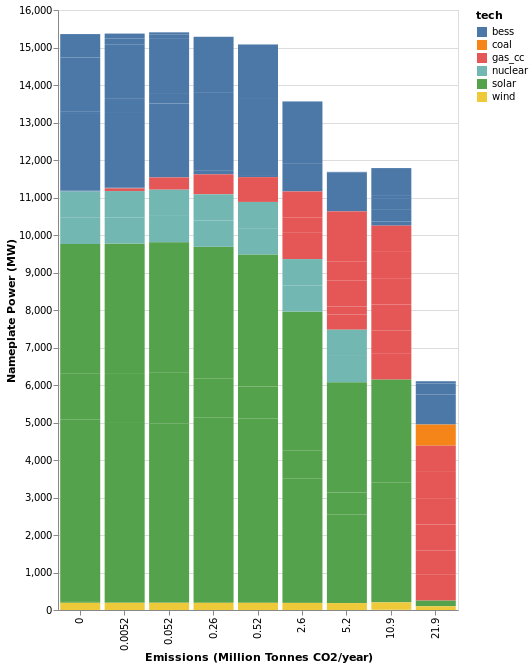
\includegraphics[width=0.9\linewidth]{Images/nameplate_power.png}
  \captionof{figure}{Nameplate power for optimal systems across different levels of emissions constraints}
  \label{fig:nameplate-power}
\end{figure}

\begin{figure}
  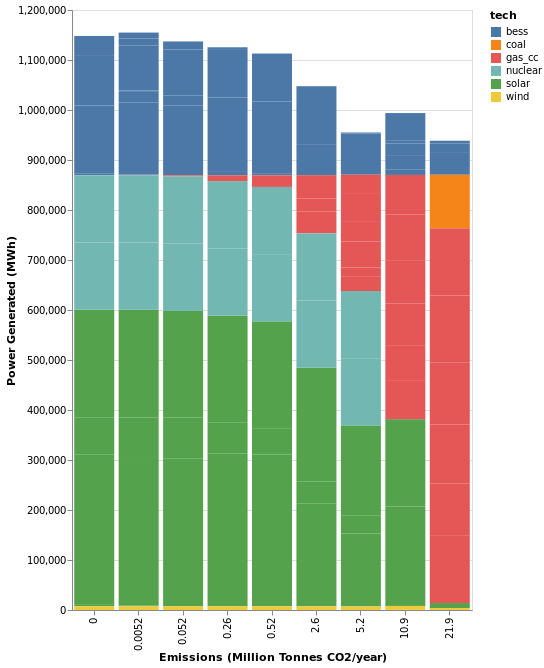
\includegraphics[width=0.9\linewidth]{Images/power_generated.png}
  \captionof{figure}{Power generated by each generationg technology across different levels of emissions constraints}
  \label{fig:power-generated}
\end{figure}

As emissions constraints are tighted, the generation mix moves increasingly towards solar and BESS technologies. Coal is phased
out with the first emissions constraint. Nuclear generation is introduced at emissions levels less than 5.2 million tonnes CO$_2$
and the capacity level remains consistent even as constraints are tightened.

Figure \ref{fig:emissions-pareto} plots the emissions pareto curve: total (annual) system cost (equation (\ref{eq:cost_func})) versus total
emissions $\epsilon$ (equation (\ref{eq:emissions})). This plot demonstrates the tradeoff between emissions and total system cost.
On a twin axis, we plot the value of the dual
variable associated with the emissions constraint (labeled as "Carbon Tax" for reasons discussed in section \ref{sec:discussion})


\begin{figure*}
  \centering
  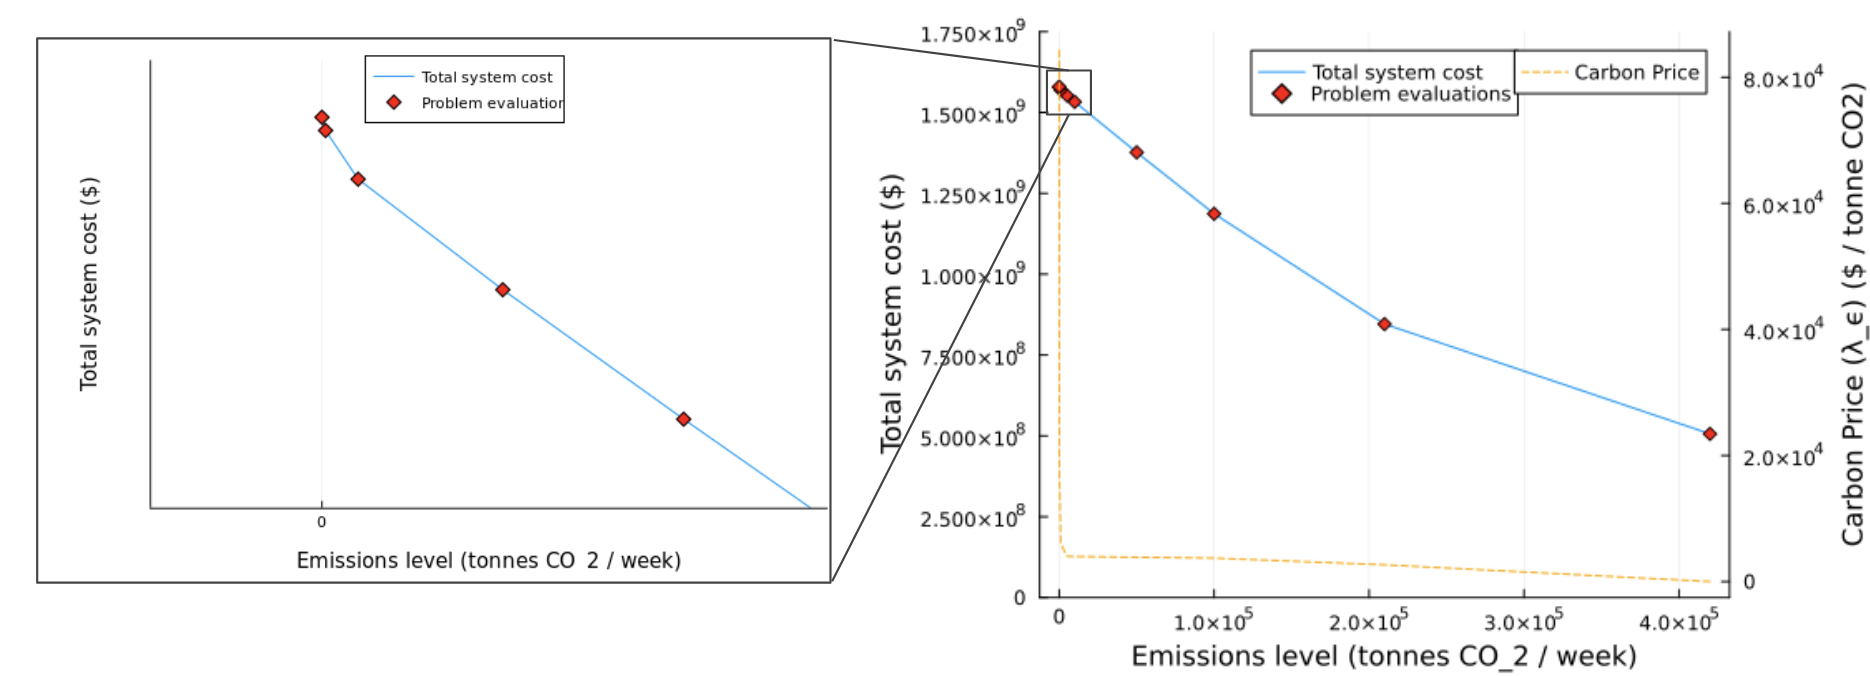
\includegraphics[width=0.9\linewidth]{Images/emissions_pareto.png}
  \captionof{figure}{Emissions Pareto Curve}
  \label{fig:emissions-pareto}
\end{figure*}

Figure \ref{fig:1} shows the dispatch result from loading the zero-emissions model back into SAint.
SAint reports that 99.9\% of load is served. Figure \ref{fig:2} shows how much solar PV capacity is allocated
to each node in the network, as well as the line loading percentage during an hour of daytime operation. A plot
of battery storage allocation is qualitatively very similar to the plot of installed PV capacity, i.e. the 
largest quantities of BESS storage are co-located on the same nodes as PV capacity.  Line loading percentages
are close to 100\% for transmission lines which connect nodes with large demand to those with solar generation.


\begin{center}
  
\includegraphics[width=0.9\linewidth]{Images/dispatch_stack.png}
  \captionof{figure}{Dispatch stack showing mix of generation resources (mostly a combination of solar and energy storage is utilized
  showing the economic viability
  )}
  \label{fig:1}
\end{center}

\begin{center}
  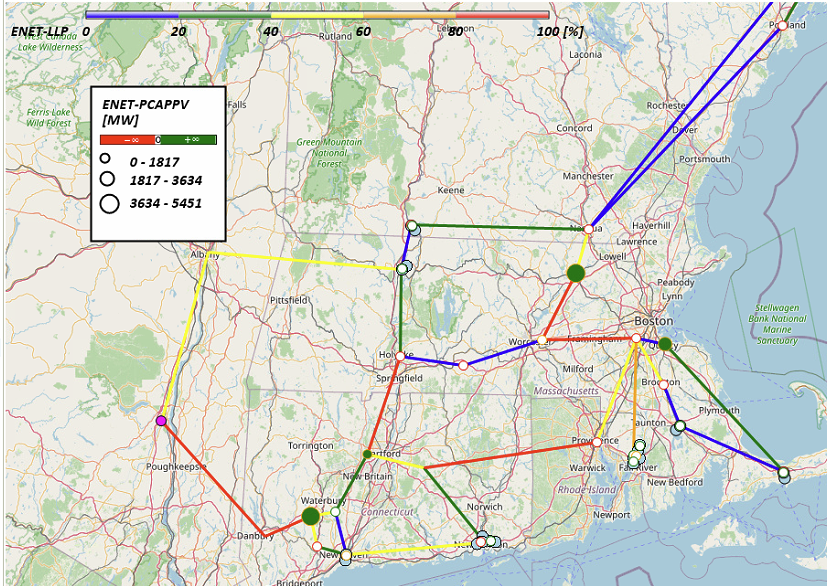
\includegraphics[width=0.9\linewidth]{Images/PV_cap.png}
  \captionof{figure}{Installed solar capacity per node (larger green dots indicate more capacity). The optimization result allocates
    relatively similar amounts of energy storage at each node with solar generation, and then smaller amounts elsewhere.
    }
  \label{fig:2}
\end{center}

\section{Discussion}
\label{sec:discussion}

The first noteworthy takeaway from figure \ref{fig:nameplate-power} is that with no emissions constraints, our model concludes that natural gas is the
most economically viable generation source. The combination of higher capital expenses and intermittency of solar and wind technologies 
seems to outweigh the benefits of their zero marginal costs. The assumed plant lifetimes of 25 years (shorter than combined cycle natural gas)
associated with solar and wind (table \ref{}) contributes to this effect. Another contributing factor is that our model does not account
for the startup and shutdown costs of operating thermal generators, the total cost in the emissions-heavy systems may be underestimated.



The emissions pareto curve of figure \ref{eq:emissions} shows a somewhat surprising result: we find the per-tonne cost of carbon
is relatively constant until the level of emissions constraints approaches very
close to zero. From emissions levels of 21.9 million tonnes/year (unconstrained case) down to 0.26 tonnes/year, the cost increases
a relatively modest amount from 2,650 \$ / million tonnes at 10.9 million tonnes/year up to just more that 4,000 \$/million tonnes
at 0.26 million tonnes/year. 

The value of this dual variable represents the sensitivity of the total system cost to a small change in the emissions constraint.
In other words, it represents the derivative of the emissions pareto curve. 

The Pareto Curve is 



\section{Conclusion}
The the theoretical problem formulation from section \ref{sec:problem} shows
show initial promise towards a unified understanding of energy storage, demand response, and
the other modern grid conceptions. Numerical results demonstrate its viability.
% \subsection{Externals}
% Incomplete...
% \subsection{Cost Functions}
% Incomplete...


\bibliographystyle{IEEEtran}
\bibliography{battery_deg.bib}



% \section{Methods}
% The mathematical formulation of section \ref{sec:problem} was implemented in using Julia and JuMP.
% To test for correctness, the author manually ran a number of test cases on a simple 3-bus system, with
% and without storage.
% 
% To assess computational scalability, the author wrote code to import encoord's ENET39 model into
% Julia. The topology of the 39-bus network is not (yet) modified.
% 
% Research was performed into BESS-pecific operational constraints and cost data has been import from EIA.
% Further test on more specific/realistic test cases is in progress.
% 
% \section{Results}
% The solution to 3-bus system abides by all operational constraints. The 39-bus system results remain to
% be processed, but the algorithm runs in approximately 1 second (with linear costs).
% 


\end{document}




% that's all folks
\end{document}


